\begin{figure}[H]
    \centering
    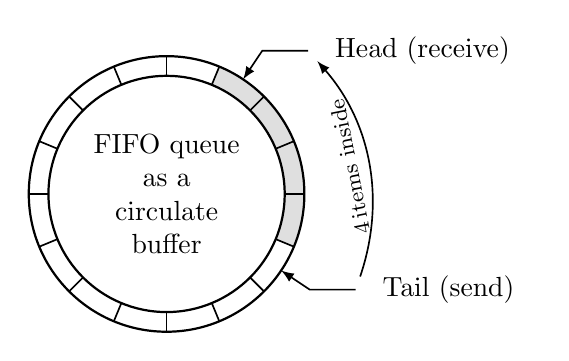
\begin{tikzpicture}[>=latex,semithick,scale=1.75]
        \fill [gray!25] (0,0) -- (67.5:1) arc [end angle=-22.5, start angle=67.5, radius=1] -- cycle;
        \draw [thick] (0,0) circle (1);
        \foreach \angle in {90,67.5,...,-67.5}
            \draw (\angle:1) -- (\angle-180:1);
        \node [circle,thick,fill=white,draw=black,align=center,minimum size=3cm] at (0,0) {FIFO queue\\ as a\\circulate \\buffer};
        \draw [<-] (56.25:1) -- (56.25:1.25) -- +(.333,0) node [right,inner xsep=.333cm] (Head) {Head (receive)};
        \draw [<-] (-33.75:1) -- (-33.75:1.25) -- +(.333,0) node [right,inner xsep=.333cm] (Tail) {Tail (send)};
        \draw [->,shorten >=5pt,shorten <=5pt] (Tail.west) to [bend right] node [midway,sloped,above,allow upside down] {\footnotesize 4\,items inside}
        (Head.west);
    \end{tikzpicture}
    \caption{qQueues conceptual representation}
    \label{fig:qqueues}
\end{figure}